%%%%%%%%%%%%%%%%%%%%%%%%%%%%%%%%%%%%%%%%%%%%%%%%%%

\chapter{Temas avanzados}

%%%%%%%%%%%%%%%%%%%%%%%%%%%%%%%%%%%%%%%%%%%%%%%%%%

Este capítulo nace de la necesidad de recojer todos los argumentos no
necesariamente ligados al uso de Matlab. La mayoría de ellos están
relacionados con la programación general o en cálculo numérico, sin
embargo son de gran utilidad para escribir buenos programas. La teoría
que contiene este capítulo es de un nivel mucho más elevado al resto,
estais avisados; esto no significa que todo esté explicado del modo
más sencillo posible.

\section{Aumentar la calidad del código escrito en Matlab}

Que el código funcione no suele ser suficiente. Debemos intentar en
cualquier caso escribir código de calidad, debemos convertir en
hábitos ciertas prácticas de programación orientadas a hacer más fácil
el uso de las funciones y los scripts. No todo termina en escribir una
pequeña ayuda en cada función. Hay estrategias muy útiles para
aumentar significativamente la potencia del código escrito sin
necesidad de aumentar el esfuerzo. Debemos entender que si Matlab es
una plataforma de desarrollo rápido de aplicaciones dispondrá de
funciones para escribir código de un modo más eficiente.

\subsection{Vectorizar, la clave para aumentar la velocidad}

Hay muchas maneras de asignar un argumento a una variable. Cuando se
crearon los ordenadores y empezaron a surgir los lenguajes de
programación casi todos los procesos eran escalares. Todo estaba
gobernado por operaciones lógicas que operaban unidades muy pequeñas
de memoria.  A medida que los ordenadores iban creciendo en potencia y
versatilidad se empezó a pensar en una manera más eficiente de
calcular. Uno de los conceptos era la vectorización.\footnote{ Un
  nombre propio en la arquitectura de ordenadores es Seymour Cray, su
  biografía está íntimamente ligada al los ordenadores vectoriales.
  Su influencia es tremenda en el campo de la computación a gran
  escala. }

Se dice que una operación es escalar cuando se hace elemento a
elemento.  Una suma escalar de dos vectores es tomar los elementos de
cada uno de ellos, sumarlos y asignar el resultado a un tercer vector.
Una operación es vectorial cuando se hace por bloques mayores en la
memoria.  Una suma vectorial de dos vectores sería tomar partes del
los vectores o los vectores enteros y sumarlos de golpe.

Los compiladores modernos son capaces de vectorizar automáticamente.
Advierten que dos bucles pueden combinarse perfectamente y realizan la
operación por bloques ahorrando memoria y tiempo de cálculo. Como
Matlab es un programa secuencial carece de esta capacidad de
optimización.  Si nosotros le pedimos un bucle con operaciones
escalares lo va a realizar sin ningún tipo de optimización. Si en
cambio asignamos operamos las matrices mediante la notación matricial
y las submatrices Matlab sí va a ser capaz de vectorizar la operación.

En la sección \ref{sub:El-truco-m=E1s} explicaremos la importancia que
todas estas consideraciones tienen sobre la velocidad de ejecución.

\subsubsection{\label{sub:El-truco-m=E1s}El truco más importante de la
  programación en Matlab}

El truco más importante para que nuestros scripts tengan una velocidad
aceptable es evitar los bucles con contador. Es la estructura más
lenta que existe en el lenguaje. El siguiente ejemplo nos ayudará a
entenderlo perfectamente. Crearemos dos matrices de números aleatorios
y las sumaremos creando una tercera matriz. Primero lo haremos
mediante un bucle que sume con dos índices y luego utilizando el
operador suma elemento a elemento. Utilizaremos la función
\texttt{rand} para crear las matrices y la pareja \texttt{tic} y
\texttt{toc} para calcular el tiempo de cálculo.

\begin{verbatim}
>> a=rand(66); #matriz de 66 x 66
>> b=rand(66);
>> tic;for i=1:66;for j=1:66;c(i,j)=a(i,j)+b(i,j);end;end;toc
ans = 0.17925
>> tic;c=a.+b;toc
ans = 0.00058100
\end{verbatim}
Donde el número que obtenemos como resultado es el tiempo transcurrido
entre la llamada de \texttt{tic} y la de \texttt{toc}. La diferencia
entre los dos métodos es de%
\footnote{El ordenador con el que han sido efectuadas las pruebas es
  un Athlon XP 2600+ (1.920 GHz, bogomips=3301.37) con 512 Mb de RAM a
  400 MHz y Octave 2.1.72. Matlab es ligeramente más rápido con el
  manejo de bucles aunque de ningún modo se acerca a la velocidad de
  los operadores matriciales. Con la optimización máxima Matlab y
  Octave tienen resultados equivalentes. Las pruebas se han efectuado
  diez veces y se da el tiempo medio de la muestra.%
}:

\begin{verbatim}
>> 0.17925/0.00058500
ans = 306.41
\end{verbatim}
Utilizar los operadores matriciales y las submatrices generará código
del orden de 100 veces más rápido. Para una EDP esto es la diferencia
entre un rato de espera y una semana de cálculos, sólo un contador mal
puesto puede acabar con un código globalmente bien escrito.

La lentitud de los bucles llega hasta límites insospechados.
Supongamos que queremos multiplicar todas las filas de una matriz por
un escalar distinto. En un alarde decidimos convertir la serie de
números en un vector y utilizar un bucle contador para operar la
matriz por filas del siguiente modo:

\begin{verbatim}
>> a=1:66;
>> b=rand(66);
>> tic;for i=1:66;c(i,:)=a(i)*b(i,:);end;toc
ans = 0.0032920
\end{verbatim}
Para eliminar este bucle tenemos que convertir la secuencia de números
en una matriz de $66\times66$ y luego multiplicarla por una matriz.
Qué sorpresa nos llevamos cuando observamos que el tiempo de proceso
es menor:

\begin{verbatim}
>> tic;c=a'*ones(1,66).*b;toc
ans = 0.00067000
\end{verbatim}
Eliminando un bucle que parecía completamente justificado acabamos de
reducir el tiempo de proceso a la décima parte.

A partir de ahora nos lo pensaremos dos veces antes de escribir la
palabra \texttt{for}. Si nos acostumbramos pensar con submatrices nos
ahorraremos tiempo de cálculo y la engorrosa tarea de migrar código a
Fortran inútilmente.

\subsubsection{¿Por qué son tan lentos los bucles?}

Lo que hace que los bucles sean tan lentos no es únicamente la
ausencia de vectorización en el cálculo.  Los bucles escalares son muy
rápidos sea cual sea la arquitectura y el lenguaje de programación.
Si analizamos con un poco más de precisión el código de los ejemplos
anteriores observamos que no sólo se están multiplicando dos matrices
o dos escalares, además se está reservando la memoria correspondiente
al resultado.

Imaginemos que queremos sumar dos vectores y asignar el resultado a un
tercero y que para ello utilicemos un bucle.  Primero tomaremos el los
primeros índices de cada vector y los situaremos en una posición de
memoria nueva.  Esto sucederá a cada paso con lo que cada iteración
implicará una operación de reserva de memoria al final de un vector.

Cada vez que ampliamos un vector \emph{llenando} una posición vacía
Matlab debe comprobar que el elemento no existe, ampliar la memoria
reservada al vector para poder situar el nuevo elemento donde debe y
rellenar el resto con ceros y finalmente almacenar los datos del nuevo
vector.

Cuando sumamos dos vectores escalarmente el ciclo de
verificación-reserva-asignación-cierre se realiza una sola vez.
Podemos concluir entonces que la operación de ampliación de una matriz
en Matlab es especialmente lenta.  Aunque no estemos obligados a
declarar las variables antes de inicializarlas es siempre una buena
práctica comprobar que cada matriz se defina entera o mediante bloques
lo suficientemente grandes.

Este comportamiento está ligado al funcionamiento de los arrays en C;
un buen texto para comprenderlo mejor es \cite{Numerical} donde
encontraremos un capítulo inicial sobre qué es verdaderamente un array
y qué relación tiene con un puntero.

Como curiosidad diremos que mientras las operaciones de reserva y
liberación de memoria son bastante lentas, las operaciones de
manipulación de forma como la función \texttt{reshape} son
especialmente rápidas.  No debemos tener miedo a cambiar la forma de
las matrices según nuestras necesidados pensando que estamos
sacrificando tiempo de ejecución.

\subsection{Control de las variables de entrada y salida en
  funciones.(+)}

La necesidad de pasar una cantidad fija de argumentos a una función en
forma de variables no es una limitación para Matlab. Uno de los puntos
débiles de la definición de las cabeceras de las funciones es que no
pueden definirse, tal como lo hacen otros lenguajes de programación,
valores por defecto para las variables de entrada. Matlab cuenta con
la siguiente serie de funciones dedicadas a manipular las variables de
entrada y salida de las funciones:

\begin{description}
\item [nargin\index{nargin}]Da el número de argumentos con el que se
  ha llamado una función
\item [nargoun\index{nargoun}]Retorna el número de argumentos de
  salida de una función
\item [varargin\index{varargin}]Permite que las funciones admitan
  cualquier combinación de argumentos de entrada.
\item [varargout\index{varargout}]Permite que las funciones adimitan
  cualquier combinación de argumentos de salida.
\item [inputname\index{inputname}]Retorna el nombre de la variable que
  se ha pasado como argumento de entrada en una función.
\end{description}
Estas funciones son una ayuda esencial cuando escribimos funciones muy
polivalentes. Los métodos \texttt{nargin} y \texttt{nargout} sirven
para que las funciones se comporten de un modo distinto según la
cantidad de argumentos que reciban, \texttt{varargin} y
\texttt{varargout} hacen que no tengamos que preocuparnos de escribir
largas cabeceras de funciones cuando estas reciben muchos argumentos,
es como si recibiera una variable tipo celda de un modo automático.


\subsection{Comunicación entre el entorno de ejecución global y el
  entorno de la función}

En el léxico utilizado por Matlab se habla de dos entornos de
ejecución o \emph{workspaces}. Existen sólo dos workspaces en los que
habitan varibles inicialmente independientes. El modo usual de
comunicar los dos entornos es mediante variables globales, una vez
definimos una variable como global en todos los \emph{workspace} la
hacemos visible para todas las unidades de programa. Matlab define dos
\emph{workspace}, base y caller. Base es el nombre del entorno de
ejecución principal; sería el intérprete en una sesión interactiva.
Caller es la función que se esté activa en algún momento de la
ejecución. Los dos métodos siguientes son interfaces entre las
variables en base y las variables en caller.

\begin{description}
\item [evalin\index{evalin}]Evalua una variable o una expresión en
  cualquier entorno.
\end{description}
Por ejemplo, vamos a crear una función que intente capturar una
variable del entorno de ejecución principal en una función. Para ello
escribiremos la siguiente función:

\begin{verbatim}
function out=testfunc()
  out=evalin('base','dummy');
\end{verbatim}
Ahora en una sesión del intérprete definiremos la variable
\texttt{var} y veremos cómo queda capturada por la sentencia
\texttt{evalin} sin que aparezca en la cabecera:

\begin{verbatim}
>> testfunc()
error: `dummy' undefined near line 23 column 1
error: evaluating assignment expression near line 2, column 4
error: called from `testfunc'
\end{verbatim}
Nos ha dado un error porque aún no hemos definido la variable
\texttt{dummy} en el entorno base. Si ahora definimos la variable y
llamamos la función:

\begin{verbatim}
>> dummy='hola'
>> testfunc()
ans = hola
\end{verbatim}
Acabamos de comuncar de un modo bastante elegante los dos entornos de
ejecución. Los programadores experimentados están acostumbrados a
lidiar con los punteros. nos podemos imaginar esta función como una
manera razonable de emular el comportamiento de un puntero%
\footnote{Un puntero es un tipo especial de variable cuya misión es
  {}``apuntar'' a una dirección de memoria, normalmente expresada por
  otra variable.  El puntero no es una variable convencional, es
  filosóficamente algo distinto. el contenido de una variable sólo
  podemos cambiarlo nosotros, en cambio el valor al que apunte el
  puntero puede cambiar si así lo exige la ejecución. El concepto de
  un puntero es abstracto y requiere comprender qué es una posición en
  la memoria física de un ordenador.  Es un concepto interesante y
  requiere comprenderlo.%
} y así añadir algo de potencia a nuestros algoritmos. No será
literalmente un puntero porque en vez de apuntar una posición de
memoria apuntará a una variable pero como es la manera normal de
definir los punteros podemos hacer que se comporte del mismo modo. Por
ejemplo, en el caso anterior hemos definido una función que extrae el
valor \texttt{out} que {}``apunta'' al valor contenido en la variable
\texttt{dummy}.  ¿Qué sucede si cambiamos la variable \texttt{dummy}?
Pues que en tiempo de ejecución la variable \texttt{out} cambiará
inmediatamente de valor:

\begin{verbatim}
>> dummy='adios'
dummy = adios
>> testfunc()
ans = adios
\end{verbatim}
Vemos que esto no es exactamente una asignación de una misma posición
de memoria pero la ejecución emula el mismo comportamiento, es como
hacer un \texttt{out==dummy} implícito.

\begin{description}

\item [assignin\index{assignin}]Asigna un valor dado a una variable de
  cualquier entorno de ejecución.
\end{description}

Estas dos funciones es el método recomendado para establecer una
comunicación entre el entorno de ejecución de las funciones y el
entorno principal.  Se sugiere sacrificar el uso de las variables
globales en favor de la asignación y la evaluación entre workspaces.
Sin embargo es una sutileza sujeta al estilo de programación.
Personalmente encuentro las variables globales mucho más intuitivas.


\section{Array Masking}

Cuando necesitamos controlar el flujo de ejecución de un programa y este
flujo necesita ciertas condiciones lógicas solemos utilizar una 
estructura condicional (\texttt{if}).  Cuando dichas condiciones lógicas
adquieren un alto grado de complejidad, con más de seis o siete opciones
que pueden ser complementarias entre ellas, la implementación de la
estructura suele ser harto complicada.

En programación suelen evitarse este tipo de estructuras, son lentas,
difíciles de programar, difíciles de entender y propensas a generar
errores en tiempo de ejecución que cuesta bastante resolver. En otros
lenguajes de programación los defectos de forma suelen ser los más
importantes pero ya hemos aprendido que en Matlab es una buena práctica
programar con la velocidad en mente.

El concepto detrás del \emph{array masking} es que, en lo que respecta
a la velocidad de ejecución, siempre será más rápido utilizar más
memoria que ahorrar en ella.  Supongamos por ejemplo que queremos
quedarnos con todos los elementos mayores a un determinado número en
una matriz dada. Será más rápido crear una matriz del tamaño de
nuestro dato y operar con ambas.

Un caso patológico del \emph{array masking} es el caso en el que
debemos seleccionar elementos de una matriz y crear con ellos otro
array de menores dimensiones. Este paso contiene todos los problemas
asociados a la pérdida de velocidad:
\begin{itemize}
\item Uso de bucles para leer elementos de una matriz
\item Una condición lógica que se evalúa para cada elemento
\item Un vector resultado que va creciendo a medida que se encuentran
  elementos que cumplen la condición.
\end{itemize}

El modo más sencillo de crear este tipo de vectores o matrices en, por
ejemplo, python son las list comprehensions que permiten crear
directamente un array con una condición lógica.  La clave para
implementar estos algoritmos de un modo eficiente en Matlab es
mediante el uso de la función \texttt{find}.

Supongamos que queremos pasar todos los elementos de un vector mayores
que cero a una nueva variable:

\begin{verbatim}
>> d = [2,-3,4,-2,3,4,-1]
d =

   2  -3   4  -2   3   4  -1

>> d(find(d>0))
ans =

   2   4   3   4
\end{verbatim}

Quizás algunos hayan visto la luz con esto.

\section{Introducción al debbugging}
Los comandos de debugging están cambiando en las últimas versiones de
octave para hacerse más parecidas a las de Matlab.

La traducción de la palabra debugging es ``quitar los bichos''.  Un
bug o bicho es un error en el código, sus efectos pueden ser evidentes
o sutiles y la tarea de encontrarlos es mucho más complicada que
eliminarlos.  Los debuggers son programas especiales para esta tarea
de uso en lenguajes compilados. Lo que hacen es ejecutar los procesos
paso a paso para conocer su funcionamiento de un modo más interactivo.
Matlab ya es en sí mismo interactivo pero algunas herramientas del
debugging clásico serán útiles en programas muy grandes.

El debugging se basa en los \emph{breakpoints} que no son más que
puntos en los que podemos detener la ejecución del programa para
analizar su estado actual. La posición de los breakpoints es más una
labor de experiencia que una ley tanto en los lenguajes compilados
como interactivos. Solemos poner uno antes de llamar una función y
unos cuantos antes de que aparezca el error.

El editor de Matlab es además el interfaz para el debugger. Podremos
poner y quitar los breakpoints con el ratón y recuperar el control del
proceso con la consola. Pero cuando uno se siente cómodo con el
debugging prefiere realizar todo el proceso manualmente mediante las
funciones propias. Estas funciones son casi las mismas en Matlab y
Octave.

\begin{description}
\item [keyboard]Esta palabra clave no es parte del debugging en
  sentido estricto pero puede ser muy útil para resolver errores del
  código.  Si introducimos esta función en un programa pararemos su
  ejecución y pasaremos a tener el control en el punto de ejecución
  donde nos encontremos. Se abrirá un intérprete mediante el cual
  accederemos al estado actual del programa para poder acceder a las
  variables de modo interactivo. Una vez salgamos del intérprete
  continuaremos la ejecución conservando los cambios que hayamos
  introducido. Este es el modo más sencillo de hacer debugging en
  scripts porque las funciones para debugging clásicas sólo operan
  dentro de funciones.
\item [{echo}] \index{echo}Traducido eco.  Controla si los comandos en
  archivos aparecen o no en pantalla. Esta sentencia sólo tiene efecto
  dentro de un archivo o de una función.  Normalmente los comandos
  ejecutables de funciones y scripts no aparecen en pantalla, sólo
  aparece su resultado si no hemos puesto un punto y coma al final de
  la línea. Con \texttt{echo on} los comandos de los scripts se
  escriben como si los hubieramos introducido a través
  del intérprete.\\
  \\
  \begin{minipage}[c]{1\linewidth}%
    \texttt{on} Activa el eco en los scripts

    \texttt{off} Desactiva el eco en los scripts

    {\texttt{on all}} Activa el eco en scripts y funciones

    {\texttt{off all}} Desactiva el eco en scripts y
    funciones\end{minipage}%

\item [type\index{type}]Saca por pantalla el texto correspondiente a
  cualquier función que esté en el árbol de directorios dentro de un
  archivo \texttt{.m}.  Es útil cuando disponemos de una colección
  propia de funciones bastante extensa y preferimos no abrir el
  archivo con el editor.
\end{description}
Como ejemplo del uso de las funciones de debugging utilizaremos el
script \texttt{polyadd.m} que implementa la suma de dos polinomios.
Las rutinas básicas para el debugging de funciones son:

\begin{description}
\item [dbtype\index{dbtype}]Muestra la función con los números de
  línea para facilitar la inclusión de breakpoints
\end{description}
Para usarlo con nuestra función sería

  \begin{verbatim}
>> dbtype polyadd
1       function poly=polyadd(poly1,poly2)
2         if (nargin != 2)
3           usage('polyadd(poly1,poly2)')
4         end
5         if (is_vector(poly1) && is_vector(poly2))
6           if length(poly1)<length(poly2)
7             short=poly1;
8             long=poly2;
9           else
10            short=poly2;
11            long=poly1;
12          end
13          diff=length(long)-length(short);
14          if diff>0
15            poly=[zeros(1,diff),short]+long;
16          else
17            poly=long+short;
18          end
19        else
20          error('both arguments must be polynomials')
21        end
\end{verbatim}
Ahora queremos colocar dos breakpoints, uno en la línea 14 y otro en
la línea 16. Para ello usaremos la siguiente función:

\begin{description}
\item [{dbstop\textsl{(func,line)}}\index{dbstop}]Introduce un
  breakpoint en una función.
\end{description}
\begin{verbatim}
>> dbstop('polyadd','14')
ans = 14
>> dbstop('polyadd','16')
ans = 17
\end{verbatim}
Fijémonos que la función no nos ha dejado poner el breakpoint en la
línea 16 porque no es ejecutable. Para comprobar el estado de la
función:

\begin{description}
\item [dbstatus]Devuelve un vector cuyos elementos son las líneas con
  breakpoints.
\end{description}
\begin{verbatim}
>> dbstatus polyadd
ans =
  14  17
\end{verbatim}
Ahora utilizamos la función del modo usual. La ejecución avanzará
hasta que encuentre un breakpoint, entonces se abrirá una consola que
nos dará el control de la ejecución.

  \begin{verbatim}
>> polyadd([3,2,1,3],[3,2,0])
polyadd: line 14, column 8
diff
debug>
\end{verbatim}
La consola \texttt{debug} es local, es decir, sólo contiene las
variables de la ejecución de la función. Lo más lógico en este punto
es utilizar la función \texttt{who} para saber qué variables han sido
iniciadas:

  \begin{verbatim}
debug> who
*** local user variables:
__nargin__   argn         long         poly1        short
__nargout__  diff         poly         poly2
\end{verbatim}
Aprovechamos para conocer algunas de ellas:

  \begin{verbatim}
debug> long
long =
  3  2  1  3
debug> poly1
poly1 =
  3  2  1  3
debug> poly2
poly2 =
  3  2  0
debug> __nargin__
__nargin__ = 2
\end{verbatim}
\texttt{\_\_nargin\_\_} es el número de argumentos de entrada. Si
salimos de la consola avanzaremos hasta el siguiente breakpoint o
finalizaremos la ejecución. En este caso llegaremos hasta la línea 17.

Para eliminar alguno de los breakpoints:

\begin{description}
\item [{dbclear\textsl{(func,line)}}\index{dbclear}]Elimina el
  breakpoint de la línea solicitada.
\end{description}
\begin{verbatim}
>> dbclear('polyadd','17')
polyadd
symbol_name = polyadd
>> dbstatus polyadd
ans = 14
\end{verbatim}
Hay más comandos para debugging pero estos son los más importantes.


\section{Optimización de la evaluación de funciones.(+)}

En la sección \ref{sub:Evaluaci=F3n-de-funciones.} hemos planteado la
necesidad de optimizar el proceso de evaluación de funciones
especialmente complejas.  El coste de la evaluación de una función muy
compleja puede reducirse significativamente con la interpolación
polinómica. Un caso muy llamativo son las funciones con gran cantidad
de términos armónicos (senos, cosenos y tangentes) que en la
evaluación suelen cancelarse. Aunque la evaluación de funciones no es
una de las tareas más optimizadas de Matlab no está de más utilizar
los conocimientos adquiridos para aumentar su rendimiento%
\footnote{Estas consideraciones no son un caso único de Matlab. El uso
  de un polinomio interpolante de alto orden para aproximar una
  función analítica es efectivo en cualquier lenguaje de programación.
  Es una práctica de optimización muy utilizada en los códigos
  antiguos escritos en fortran cuando los compiladores no eran
  suficientemente listos como para evaluar las funciones de un modo
  eficiente. Los códigos altamente optimizados no tenían ninguna
  función que no estuviera escrita \emph{a mano} por el programador.
  Los tiempo en los que cada \emph{flop} era valioso ya han pasado
  pero siempre podemos encontarnos en la necesidad de optimizar una
  función en concreto%
}. Los polinomios de Chebyshev son un recurso bastante habitual porque
implican un error de interpolación pequeño. También podríamos pensar
en utilizar un desarrollo de Taylor, pero tienen el inconveniente de
que sólo aproximan la función en un punto, mientras que lo que nos
interesa es un error controlable en todo un intervalo.

Otra característica interesante es que cuando desarrollamos una
función en serie, ya sea de Fourier o Polinómica, las operaciones
elementales como las derivadas o las integrales son triviales y, lo
que es más importante, fáciles de implementar%
\footnote{El grado de optimización en los inicios de la informática
  era tal que en un mismo bucle se aprovechaban los términos
  calculados para la evaluación de una función para evaluar a la vez
  su derivada; en el caso que fuera necesario.%
}.


\subsection{Polinomios de Chebyshev.}

\emph{Este es un resumen del tratamiento del desarrollo en polinomios
  de Chebyshev hecho en \cite{Numerical}.}

Los polinomios de Chebyshev cumplen la siguiente formula:
$$T_{n}(x)=\cos(n\ \cos^{-1}x)$$
Esta expresión genera la siguiente serie de polinomios:
$$ T_{0}(x)=1$$
$$
T_{1}(x)=x$$
$$
T_{2}(x)=2x^{2}-1$$
$$
T_{3}(x)=4x^{3}-3x$$
$$
T_{4}(x)=8x^{4}-8x^{2}+1$$
$$
\cdots$$
$$
T_{n+1}(x)=2xT_{n}(x)-T_{n-1}(x)\qquad n\geq1$$


\begin{itemize}
\item Estos polinomios tienen la particularidad de contar con $n$
  ceros en los puntos:
$$x=\cos\left(\frac{\pi(k-1/2)}{n}\right)\qquad
k=1,2,\ldots,n$$ y $n+1$extremos relativos en:
$$  x=\cos\left(\frac{\pi k}{n}\right)$$
acotados por el intervalo $[-1,1]$. Estos polinomios, además, tienen
la característica de ser ortogonales según la función peso
$(1-x^{2})^{-1/2}$.  Se demuestra que los coeficientes del desarrollo
de la forma:
$$
f(x)\approx\sum_{k=-1}^{N}c_{k}T_{k-1}(x)-\frac{1}{2}c_{1}$$ se
calculan mediante:
$$  c_{j}=\frac{2}{N}\sum_{k=1}^{N}f
\left( \cos\left(\frac{\pi(k-1/2)}{N}\right) \right)
\cos\left(\frac{\pi(j-1)(k-1/2)}{N}\right)$$

\end{itemize}
Evidentemente no necesariamente nos interesa un desarrollo que
contenga todos los puntos posibles; lo más normal es calcular un
desarrollo truncado de Chebyshev. Con el cambio de variable$$
y\equiv\frac{x-\frac{1}{2}(b+a)}{\frac{1}{2}(b-a)}$$ conseguimos un
desarrollo en el intervalo $[a,b]$, mucho más útil que el $[-1,1]$
original.

La siguiente es una función escrita en C++ que implementa el
desarrollo.  Es interesante fijarse en cómo escribir la ayuda en
formato \textit{texinfo}

\begin{verbatim}
/* chebyexpand.cc */
#include <octave/oct.h>
#include <math.h>

static double PI=4.*atan(1.);

DEFUN_DLD(chebyexpand,args, ,
"-*- texinfo -*-\n\
@deftypefn {Loadable Function} {[@var{c}]=} chebyexpand\
(@var{f},@var{a},@var{b},@var{n})\n\
\n\
Chebyshev fit:\n\
\n\
Given a function @var{f} and the interval @var{a},@var{b} computes\n\
the @var{n} coefficients of the Chebyshev polynomial expansion.\n\
\n\
@example\n\
>> chebyexpand(@@(x) 2*x^2-1,-1,1,5)\n\
ans =\n\
   -2.6645e-16\n\
    1.1948e-17\n\
    1.0000e+00\n\
    7.9786e-17\n\
   -1.0426e-16\n\
@end example\n\
\n\
Note that @var{f} must be a function handle or an anonymous function\n\
\n\
@end deftypefn")
{
  int j,k;

  octave_value_list tmp;
  octave_value_list inval;
  octave_function *input_fcn=0;

  if (args(0).is_function_handle() || args(0).is_inline_function())
    input_fcn = args(0).function_value();
  else
    {
      error("this is not a function handle nor an inline function");
      return octave_value(-1);
    }

  double a=args(1).double_value();
  double b=args(2).double_value();
  int n=args(3).int_value();

  ColumnVector f=ColumnVector(n);
  ColumnVector c=ColumnVector(n);

  for (k=0;k<n;k++)
    {
      inval(0)=octave_value(cos(PI*(k+0.5)/n)*\
                            0.5*(b-a)+0.5*(b+a));
      tmp=input_fcn->do_multi_index_op(1,inval);
      f(k)=tmp(0).double_value();
    }
  for (j=0;j<n;j++)
    {
      double sum=0.;
      for (k=0;k<n;k++)
        {
          sum += f(k)*cos(PI*j*(k+0.5)/n);
        }
      c(j)=sum*2./n;
    }

  return octave_value(c);
}
\end{verbatim}

Como ejemplo de cómo debe ser la ayuda de una función de octave iremos
al intérprete y teclearemos:

\begin{verbatim}
 -- Loadable Function: [C]= chebyexpand (F,A,B,N)
     Chebyshev fit:

     Given a function F and the interval A,B computes the N
     coefficients of the Chebyshev polynomial expansion.

          >> chebyexpand(@(x) 2*x^2-1,-1,1,5)
          ans =
             -2.6645e-16
              1.1948e-17
              1.0000e+00
              7.9786e-17
             -1.0426e-16

     Note that F must be a function handle or an anonymous function
\end{verbatim}

Ahora nos falta crear la función que dados los coeficientes nos
recupere el valor de la función de un modo eficiente. Para ello
utilizamos la siguiente recurrencia también definida en
\cite{Numerical}:
$$d_{m+2}\equiv d_{m+1}\equiv0$$
$$d_{j}=2xd_{j+1}-d_{j+2}+c_{j}\qquad j=m,m-1,\ldots,2$$
$$f(x)\equiv d_{0}=d_{2}-d_{3}+\frac{1}{2}c_{1}$$ Pero una función
recurrente nos obliga a implementar un bucle, algo que rompe
completamente el objetivo de crear una función que sea muy rápida. Sin
embargo el esfuerzo de programarla en cualquier otro lenguaje es
mínimo%
\footnote{Octave cuenta con la función cheb.m pero está escrita en
  código Matlab.%
}. Por ejemplo, en C++ para octave (crear un archivo .mex sería aún
más fácil): \emph{El programa tiene un bug}

\begin{verbatim}
#include <octave/oct.h>
DEFUN_DLD(chevyval,args, ,
    "Calcula el valor del desarrollo de Chevyshev en x")
    {
        ColumnVector c (args(0).vector_value());
        double a (args(1).double_value());
        double b (args(2).double_value());
        double x (args(3).double_value());
        double xx;
        double y;
        double ynm1;
        double dummy;
        int i;
        int n =c.length();
        xx=(2.*x-a-b)/(b-a);
        if ((x-a)*(x-b)>0)
        {
            error("chevyval: bad input point");
            return octave_value_list();
        }
        else
        {
            ynm1= c(n-1);
            y=2.*xx*ynm1+c(n-2);
            for (i=n-3;i<0;i--)
            {
                dummy=y;
                y=2.*xx*y+ynm1+c(i);
                ynm1=dummy;
            }
            y=xx*y-ynm1+0.5*c(0);
            return octave_value(y);
        }
    }
\end{verbatim}


\section{OCTS (Octave Control Theory Suite)}

El control automático es una de las disciplinas más importantes de
la ingeniería de sistemas. Se aplica tanto a la aeronautica, el diseño
de sistemas mecánicos, el control de redes... Es además una herramienta
bastante sencilla con resultados sorprendentes.

A medida que el sistema de control va creciendo se complica su tratamiento
analítico pero tratandose de polinomios es sencillo diseñar herramientas
numéricas para ello. Cuando afrontamos un problema de control automático
solemos empezar con su representación en un diagrama de bloques. Cada
uno de los bloques representa una parte de las ecuaciones en forma
de funciones de transferencia y encontrar un modo sencillo de crear,
manipular y calcular el sistema no es más que un problema de diseño.

Encontramos bastantes programas especializados en el tratamiento de
sistemas dinámicos. Podemos dividirlos en dos tipos, las herramientas
por línea de comandos y las herramientas gráficas. Las primeras suelen
ser tanto o más potentes que las segundas pero su curva de aprendizaje
es más larga, incluso puede ser que demasiado larga. En el segundo
grupo nos encontramos un programa verdaderamente popular construido
sobre Matlab, Simulink.

Simulink fue creado para el tratamiento fácil de sistemas dinámicos
pero rápidamente se convirtió en una herramienta de modelado verdaderamente
potente. Casi cualquier programa de Matlab puede ser planteado en
un diagrama de bloques de Simulink. Diríamos que es la extensión natural
de los problemas de control aplicados a Matlab. Simulink es una herramienta
fabluosa pero no es parte del lenguaje de programación. Es una aplicación,
no una extensión del lenguaje.

Mantener los programas de simulación en el {}``espacio del código
fuente'' suele ser una práctica bastante beneficisa pero requiere
tiempo de desarrollo y experiencia. Este curso pretende ser una ayuda
precisamente para adquirir rápidamente esta experiencia. La manipulación
de sistemas dinámicos puede ser un buen ejemplo de cómo programar
bien en Matlab.

No analizaremos Simulink. Para esto están los libros de Simulink.
A cambio trataremos uno de los toolkits más útiles y peor documentados
de Octave, La Suite de Teoría del Control de Octave (OCTS).


\subsection{La representación del sistema}

Cada parte de un sistema dinámico puede ser expresada de muchas
maneras, en forma de función de transferencia, en el espacio de las
variables de estado y proporcionando sus ceros y sus polos.

Una de las particularidades del OCTS es que almacena cada parte del
sistema en una estructura de datos. La consecuencia directa de este
planteamiento es que para interactuar con lo almacenado estamos
obligados a utilizar las funciones diseñadas para ello:

\begin{description}
\item [tf\index{tf}]Crea un bloque mediante su función de
  transferencia
\item [ss\index{ss}]Crea un bloque mediante su representación en el
  espacio de sus variabels de estado
\item [zp\index{zp}]Crea un bloque mediante la información
  proporcionada por sus ceros y sus polos
\end{description}
El propio proceso de creación se encarga de calcular las
representaciones alternativas y almacenarlas dentro de la estructura.
Por ejemplo, para introducir:
$$block(s)=\frac{K(s+0.5)(s+1)}{s^{2}(s+0.1)(s+5)(s+10)}$$
con $K=1$
\begin{verbatim}
    >> block=zp([-0.5,-1],[-0.1,-5,-10,0,0],1)
\end{verbatim}
El resultado es el siguiente sistema
\begin{verbatim}
block =
{
  inname =
  {
    [1,1] = u_1
  }

  k = 1
  n = 5
  nz = 0
  outname =
  {
    [1,1] = y_1
  }
  pol =

     -0.10000   -5.00000  -10.00000    0.00000    0.00000

  stname =

  {
    [1,1] = x_1
    [1,2] = x_2
    [1,3] = x_3
    [1,4] = x_4
    [1,5] = x_5
  }

  sys =

    1  0  1  0

  tsam = 0
  yd = 0
  zer =

    -0.50000  -1.00000

}
\end{verbatim}

\begin{description}
\item [sysout\index{sysout}]Muestra las distintas representacoiones
  del sistema:
\end{description}
Esta función es bastante útil para conocer funciones en tiempo real.
Como ya está todo almacenado dentro de la estructura de datos del
sistema no tenemos más que solicitar cualquiera de ellas:
\begin{verbatim}
>> sysout(block,'tf')
Input(s)
      1: u_1

Output(s):
     1: y_1

transfer function form:
1*s^2 + 1.5*s^1 + 0.5
-----------------------------------------------
1*s^5 + 15.1*s^4 + 51.5*s^3 + 5*s^2 + 0*s^1 + 0

>> sysout(block,'zp')
Input(s)
      1: u_1

Output(s):
     1: y_1

zero-pole form:
1 (s + 0.5) (s + 1)
------------------------------
s^2 (s + 0.1) (s + 5) (s + 10)

>> sysout(block,'ss')
Input(s)
      1: u_1

Output(s):
     1: y_1

state-space form:
5 continuous states, 0 discrete states
State(s):
    1: x_1
    2: x_2
    3: x_3
    4: x_4
    5: x_5

A matrix: 5 x 5
  -10.00000   -4.50000    1.00000    0.00000    0.00000
    0.00000   -5.00000    1.00000    0.00000    0.00000
    0.00000    0.00000   -0.10000    1.00000    0.00000
    0.00000    0.00000    0.00000    0.00000    1.00000
    0.00000    0.00000    0.00000    0.00000    0.00000
B matrix: 5 x 1
  0
  0
  0
  0
  1
C matrix: 1 x 5
  -9.00000  -4.50000   1.00000   0.00000   0.00000
D matrix: 1 x 1
0
\end{verbatim}


\subsection{Diagramas de Bloques}

\label{sec:DiagramasBloques}

La representación por diagramas de bloques es una parte esencial de la
teoría de control. Es lo que da una idea intuitiva del sistema, un
buen diagrama de bloques es una parte muy importante del problema.
Podríamos pensar que para crear y manipular un diagrama de bloques es
estrictamente necesario una herramienta gráfica. Esto es completamente
falso como veremos a continuación. Uno de los principios de la
programación es que las estructuras deben expresarse en el código pero
no deben estar contenidas en él. No es difícil convertir
intuitivamente un bloque en un objeto con una función de transferencia
y unas entradas y salidas asociadas. Esto es precisamente lo que
tenemos que intentar programando con el OCTS.

Con los métodos de la sección anterior hemos aprendido a introducir la
función de transferencia en un bloque pero si queremos que
introducirlo en un sistema dinámico tendremos que etiquetar sus
entradas y salidas convenientemente.

Supongamos que tenemos un bloque con la siguiente función de
transferencia.
$$dcha1(s)=\frac{1}{2s+4}$$ Al bloque decidimos llamarlo {}``dhca1'' por
su posición en el hipotético diagrama de bloques. Un ejemplo de bloque
bien definido sería: %
\footnote{La constante \texttt{TSAM} no es más que el tiempo de
  muestreo. En el caso de sistemas continuos \texttt{TSAM} es igual a
  cero.%
}

\begin{verbatim}
  >> dcha1=tf([1,0],[2,4],TSAM=0,'dcha1in','dcha1out')
\end{verbatim}
Evidentemente los bloques definidos por sus funciones de transferencia
o por sus ceros y sus polos tendrán sólo una entrada y una salida.

Una vez hemos visto cómo crear bloques elementales pasamos a conocer
las funciones que permiten a los bloques interacturar entre ellos.
Son las siguientes:

\begin{description}
\item [Operaciones~aritméticas~de~bloques]:

  \begin{description}
  \item [sysadd\index{sysadd}]Combina dos bloques en paralelo de modo
    que la salida del conjunto es la suma de ambos. Para comprender
    mejor el cálculo revisar la ayuda de la función
  \item [sysmult\index{sysmult}]Combina dos bloques en serie de modo
    que la salida del conjunto es el producto de ambos
  \item [syssub\index{syssub}]Combina dos bloques en paralelo de modo
    que la salida del conjunto es la resta de ambos
  \end{description}
\item [Operaciones~de~comunicación~entre~bloques]:

  \begin{description}
  \item [sysconnect\index{sysconnect}]Conecta dos bloques definiendo
    una puerta de cada uno de ellos. Una puerta es una entrada o una
    salida de un bloque cualquiera.
  \item [sysgroup\index{sysgroup}]Agrupa varios bloques en uno que
    conserva sus entradas y salidas.
  \item [sysdup\index{sysdup}]Duplica las salidas y las entradas de un
    bloque.
  \item [sysprune\index{sysprune}]Elimina las entradas y las salidas
    espúreas del sistema
  \item [sysidx\index{sysidx}]Extrae los nombres de las puertas de un
    bloque.  Muy útil cuando se utiliza con \texttt{sysconnect}.
  \item [sysappend\index{sysappend}]Introduce nuevas puertas de
    entrada o salida a un bloque ya existente
  \item [buildssic\index{buildssic}]Constructor de sistemas dinámicos.
    Para aprender más sobre esta función es necesario utilizar la demo
    de creación de sistemas, \texttt{bddemo}.
  \end{description}
\end{description}

\subsubsection{Ejemplo de aplicación. Un sistema realimentado simple}

\label{sec:EjRealimentado}

Las ayudas de las funciones de listadas en la sección anterior son
bastante explicativas pero sin un conocimiento aproximado de un kit de
análisis de sistemas dinámicos puede costarnos dar el primer paso.

Una de las pocas consideraciones a tener en cuenta es que no se pueden
acoplar ramas en los diagarmas de bloques, tenemos que crear las
uniones duplicando las entradas y salidas en los mismos bloques. Esto
es porque en cualquier kit de análisis las ramas no son más que
conexiones, no tienen ninguna identidad propia. También debemos tener
en cuenta que hay operaciones que se realizan entre bloques del mismo
sistema y operaciones entre sistemas. Si bien \texttt{sysprune},
\texttt{sysdup} y \texttt{sysconnect} sólo permiten operar en el mismo
sistema, \texttt{sysadd} o \texttt{sysmult} relacionan dos bloques
independientes.

Para ver todo lo anterior aplicado nada mejor que un ejemplo.
Supongamos que tenemos el siguiente sistema dinámico expresado por la
figura \ref{cap:DBloques} con $F=\frac{10}{s^{2}(s+3)}$ y $G=s+2$:

%
\begin{figure}

  \centering{} 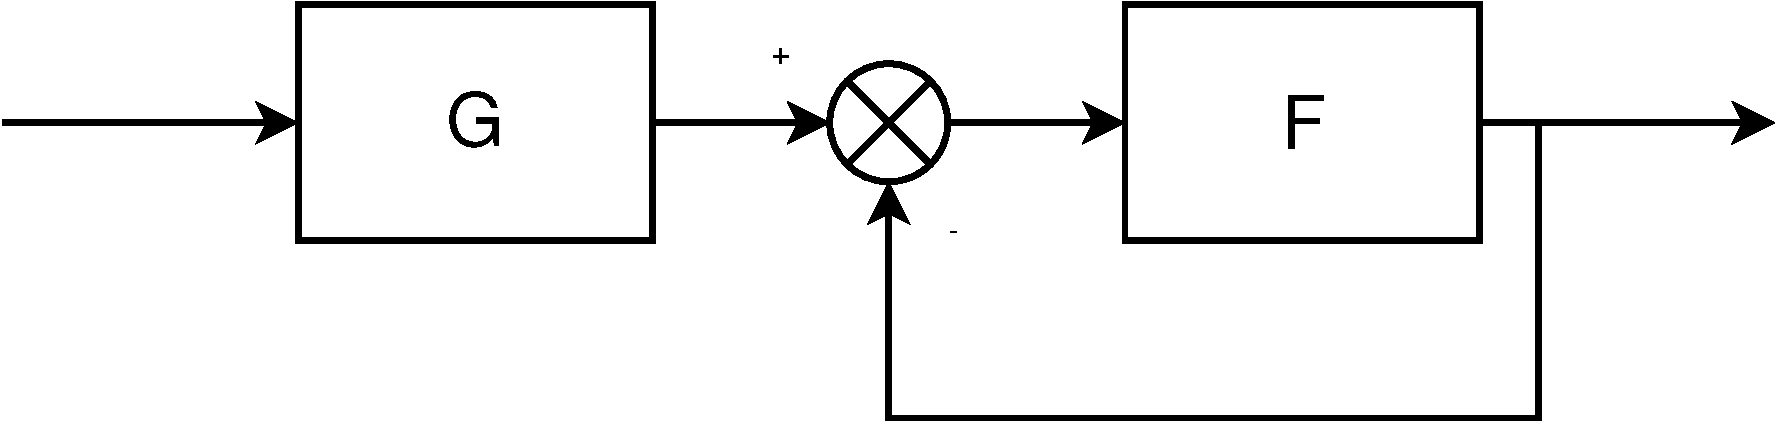
\includegraphics[width=8cm,
  keepaspectratio]{figuras/sistema1}



  \caption{\label{cap:DBloques}Diagrama de bloques del sistema
    ejemplo}
\end{figure}


Primero construiremos el bloque de la derecha, el más cercano a la
salida. Su función de transferencia es:
$DCHA(s)=\frac{10}{s^{2}(s+3)}$ de modo que empezaremos definiendo su
bloque básico:
\begin{verbatim}
>> DCHA=zp([],[0,0,-3],10,TSAM=0,'DCHAIN','DCHAOUT');
\end{verbatim} El paso siguiente es duplicar su salida 
\begin{verbatim}
>> DCHAdup=sysdup(DCHA,[],'DCHAIN');
DCHAdup =
{
  a =

    -3   1   0
     0   0   1
     0   0   0

  b =

    0  0
    0  0
    1  1

  c =

    10   0   0

  d =

    0  0

  inname =

  {
    [1,1] = DCHAIN
    [1,2] = DCHAIN(dup)
  }

  n = 3
  nz = 0
  outname =

  {
    [1,1] = DCHAOUT
  }

  stname =

  {
    [1,1] = x_1
    [1,2] = x_2
    [1,3] = x_3
  }

  sys =

    2  0  0  1

  tsam = 0
  yd = 0
}

\end{verbatim}
Como vemos ha aparecido una nueva entrada llamada
\texttt{DCHAIN(dup)}, copia de \texttt{DCHAIN}. Ahora ya podemos crear
la recirculación del primer estadio no sin antes cambiar el signo de
la nueva puerta de salida:
\begin{verbatim}
>> DCHAdup=sysscale(DCHAdup,[],diag([1,-1]));
\end{verbatim} 
Este es un modo abrevidado de utilizar la función \texttt{syscale},
consultando la ayuda aprenderemos a utilizarla de un modo más
intuitivo.  Ahora conectamos la señal a la salida con la nueva puerta
de entrada y finalmente simplificamos el sistema par que tenga una
única entrada.  Como paso final comprobaremos que el resultado es
realmente el deseado escribiendo la función de transferencia del
sistema.

\begin{verbatim}
>> DCHAend=sysconnect(DCHAdup,'DCHAOUT','DCHAIN(dup)');
>> DCHAend=sysprune(DCHAend,'DCHAOUT','DCHAIN');
>> sysout(DCHAend,'tf')
Input(s)
      1: DCHAIN

Output(s):
     1: DCHAOUT

transfer function form:
10
----------------------------------
1*s^3 + 3*s^2 + 1.554e-15*s^1 + 10
\end{verbatim} 

La definición del bloque de la izquierda es la única limitación del
OCTS. No puede definir bloques cuyo número de ceros sea mayor a su
número de polos. Esto es debido a la forma que tiene de hacer los
cálculos internos para crear la estructura de datos. Para seguir con
el ejemplo tendremos que romper la estructura de datos creada por el
primer bloque con recirculación, multiplicarla por el polinomio del
bloque de la izquierda y finalmente crear la última recirculación.
Esto no significa ningún problema porque podemos pasar de la
representación como estructura a función de transferencia sólo con
aplicar la función \texttt{sys2tf}
\begin{verbatim}
>> [num,den]=sys2tf(DCHAend);
\end{verbatim} 
Para multiplicar el numerador de la función de transferencia por el
nuevo término utilizamos la función \texttt{conv} que ya vimos en la
sección dedicada al cálculo con polinomios.
\begin{verbatim}
>> num=conv([1,2],num);
\end{verbatim} 
El paso siguiente es reconvertir la función de transferencia en el
tipo estructura.
\begin{verbatim}
>> TOTAL=tf(num,den,TSAM=0,'IN','OUT');
>> sysout(TOTAL,'tf')
Input(s)
      1: IN

Output(s):
     1: OUT

transfer function form:
10*s^1 + 20
----------------------------------
1*s^3 + 3*s^2 + 1.554e-15*s^1 + 10
\end{verbatim}


\subsection{Análisis en frecuencia}

\label{sec:analisis}

De nada servirían todas las funciones de construcción de bloques si
luego no podemos analizar el comportamiento de nuestro sistema. Esta
parte del toolkit es sin duda su punto fuerte.

Una de las pocas cosas que debemos tener en cuenta es que el sistema
que se estáresolviendo cuando se hace el análisis en frecuencias no
es el original sino el de la figura \ref{cap:DBloques2}:

%
\begin{figure}

 \centering{} 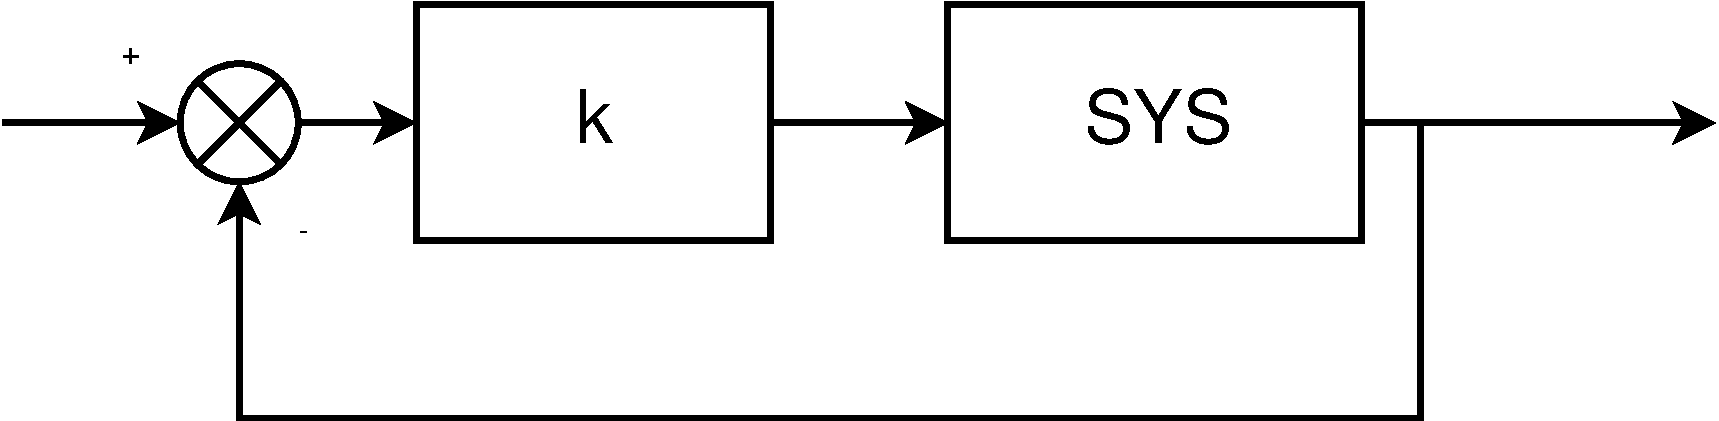
\includegraphics[width=8cm, keepaspectratio]{figuras/sistema2}


\caption{\label{cap:DBloques2}Diagrama de bloques resuelto}
\end{figure}


\begin{description}
\item [bode\index{bode}]Hace el análisis bode del sistema. En el caso
que no se soliciten argumentos de salida se dibuja el diagrama bode 
\item [nyquist\index{nyquist}]Hace el análisis nyquist de sistema. 
\item [nichols\index{nichols}]Hace en análisis nichols del sistema. 
\end{description}

\subsubsection{Ejemplo de análisis en frecuencia}

\label{sec:ejercicioanalisis} Aprovechando que ya hemos creado un
sistema en la sesión para hacer el diagrama de Nyquist basta con:
\begin{verbatim}
>> nyquist(TOTAL)
\end{verbatim} Lo que genera la figura (\ref{fig:nyquist}). %
\begin{figure}[!h]
 \centering
    \includegraphics[width=12cm, keepaspectratio]{figuras/nyquistplot}


\caption{\label{fig:nyquist}Diagrama de Nyquist del sistema}
\end{figure}


Los diagramas de bode son igualmente sencillos de conseguir (figura
\ref{cap:bode}): 
\begin{verbatim}
>> bode(TOTAL)
\end{verbatim}%
\begin{figure}
 \centering
    \includegraphics[width=12cm, keepaspectratio]{figuras/bodeplot}

\caption{\label{cap:bode}Gráfica bode del sistema}
\end{figure}

\section{Análisis Numérico de Ecuaciones en Derivadas Parciales}

Muchos problemas físicos pueden describirse mediante ecuaciones en
derivadas parciales: la transmisión del calor, el movimiento de los
fluidos, la resistencia de los materiales, la probabilidad que tiene
un electrón de estar en un orbital alrededor del núcleo.
Desgraciadamente pocas ecuaciones en derivadas parciales tienen
solución analítica.  En algunos casos, como las ecuaciones de
Navier-Stokes que describen el movimiento de un fluido no se ha
llegado ni a demostrar la existencia y unicidad de la solución.

Sin embargo sí podemos resolverlas numéricamente con más o menos
dificultades. El abanico de ecuaciones es tan amplio como los métodos
para resolverlas.

Sería una estupidez intentar abreviar aquí toda una rama de la
matemática aplicada así que me limitaré a escribir un par de
ejemplos de cómo se utilizaría el lenguaje Matlab para resolver
ciertos casos reales.

\subsection{Resolución de la ecuación del calor con simetría axial por
  volúmenes finitos en un cilindro.}


La ecuación del calor no estacionaria para un volúmen de control sin
término convectivo se puede escribir como:\[
\partial_{t}U=-\vec{q}\cdot\vec{n}\]
La variación temporal (positiva) de energía interna es igual al flujo
de calor entrante a través de su frontera descrita por el vector normal
saliente. La expresión de la energía interna es:\[
U=\int_{V}cT\ dm=\int_{V}\rho cT\ dV\]
y la del flujo de calor:\[
\vec{q}=-\int_{\partial V}k\nabla T\ dS\]
En todos los cálculos sucesivos se supondrá un volúmen finito centrado
en la celda compuesto por una porción radial del tubo. En él sólo
se considerará el gradiente radial de temperaturas. Combinando las
ecuaciones anteriores se obtiene la ecuación para el volumen de control:\[
\partial_{t}\int_{V}\rho cT\ dV=\vec{n}\cdot k\int_{\partial V}\nabla T\ dS\]
Agrupando todas las constantes y simplificando las integrales debido
a la simetría cilíndrica:\[
\frac{\rho c}{k}\partial_{t}T\int_{V}\ dV=\vec{n}\cdot\nabla T\int_{\partial V}\ dS\]
Y resolviendo las integrales por unidad de longitud del cilindro,
donde $\int_{V}dV\simeq2\pi r\ dr$ , $\int_{\partial V}dS=2\pi r$
, $\nabla T=\partial_{r}T$ y $C_{T}=\frac{\rho c}{k}$:\[
C_{T}\partial_{t}T\ r\ dr=r_{e}\partial_{r}T|_{r_{e}}-r_{i}\partial_{r}T|_{r_{i}}\]
El último paso antes de la resolución numérica es discretizar espacialmente
la ecuación con $dr=\Delta r_{j}$ y $r=r_{j}$ teniendo en cuenta
que el elemento está centrado en el cuerpo.\[
C_{T}(\partial_{t}T_{j})r_{j}\Delta r_{j}=r_{e}\left.\frac{\Delta T}{\Delta r}\right|_{r_{e}}-r_{i}\left.\frac{\Delta T}{\Delta r}\right|_{r_{i}}\]
Siguiendo con la discretización ($\Delta r_{j}=\frac{r_{j+1}-r_{j-1}}{2}$,$r_{e}=\frac{r_{j+1}+r_{j}}{2}$,$r_{i}=\frac{r_{j}+r_{j-1}}{2}$,$\left.\frac{\Delta T}{\Delta r}\right|_{r_{e}}=\frac{T_{j+1}-T_{j}}{r_{j+1}-r_{j}}$
y $\left.\frac{\Delta T}{\Delta r}\right|_{r_{i}}=\frac{T_{j}-T_{j-1}}{r_{j}-r_{j-1}}$):\[
\partial_{t}T_{j}=\frac{2}{C_{T}r_{j}}\frac{1}{r_{j+1}-r_{j-1}}\left(\frac{r_{j+1}+r_{j}}{2}\frac{T_{j+1}-T_{j}}{r_{j+1}-r_{j}}-\frac{r_{j}+r_{j-1}}{2}\frac{T_{j}-T_{j-1}}{r_{j}-r_{j-1}}\right)\]
Suponiendo una discretización equiespaciada:\[
\partial_{t}T_{j}=\frac{1}{C_{T}r_{j}}\frac{1}{\Delta r^{2}}\left(\left(r_{j}+\frac{\Delta r}{2}\right)(T_{j+1}-T_{j})-\left(r_{j}-\frac{\Delta r}{2}\right)(T_{j}-T_{j-1})\right)\]
y finalmente:\[
\partial_{t}T_{j}=\frac{1}{C_{T}\Delta r^{2}}\left(\left(1+\frac{\Delta r}{2r_{j}}\right)T_{j+1}-2T_{j}+\left(1-\frac{\Delta r}{2r_{j}}\right)T_{j-1}\right)\]
Llegamos a una expresión que puede ser integrada en el tiempo numéricamente.
De modo que el sistema de ecuaciones resultante es:\[
d_{t}T_{j}=\frac{1}{C_{T}\Delta r^{2}}\left[\begin{array}{ccccc}
\cdots &  &  &  & 0\\
 & \ddots\\
 & 1-\frac{\Delta r}{2r_{j}} & -2 & 1+\frac{\Delta r}{2r_{j}}\\
 &  &  & \ddots\\
0 &  &  &  & \cdots\end{array}\right]T_{j}\]
que a partir de ahora se expresará como \[
\dot{T}=AT\]


Los elementos del contorno tendrán además la contribución de el calor
que reciben por convección:\[
\vec{q}_{conv}=\int_{\partial V}h(T_{\infty}-T)dS=\bar{h}(T_{\infty}-T)_{\partial V}\int_{\partial V}dS\]
Entonces, para el elemento del interior del tubo y teniendo en cuenta
que su espesor es de la mitad que los elementos interiores porque
está centrado en la cara.

\[
(1/2)C_{T}\partial_{t}T\ r\ dr=r_{e}\partial_{r}T|_{r_{e}}+r_{i}\frac{h_{i}}{k}(T_{i}-T_{1})\]
\[
\partial_{t}T_{1}=\frac{2}{C_{T}\Delta r^{2}}\left(\left(1+\frac{\Delta r}{2r_{1}}\right)T_{2}-\left(2+\frac{h_{i}}{k}\right)T_{1}+\Delta r^{}\frac{h_{i}}{k}T_{i}\right)\]
y para el del exterior, también con la mitad de espesor:\[
(1/2)C_{T}\partial_{t}T\ r\ dr=r_{e}\frac{h_{e}}{k}(T_{e}-T_{N})-r_{i}\partial_{r}T|_{r_{i}}\]
\[
\partial_{t}T_{N}=\frac{2}{C_{T}\Delta r^{2}}\left(\Delta r\frac{h_{e}}{k}T_{e}-\left(2+\frac{h_{e}}{k}\right)T_{N}+\left(1-\frac{\Delta r}{2r_{N}}\right)T_{N-1}\right)\]


Con lo que la matriz del sistema es:\[
d_{t}T_{j}=\frac{1}{C_{T}\Delta r^{2}}\left[\begin{array}{ccccc}
-4-2\Delta r\frac{h_{i}}{k} & 2+\frac{\Delta r}{r_{j}} &  &  & 0\\
 & \ddots\\
 & 1-\frac{\Delta r}{2r_{j}} & -2 & 1+\frac{\Delta r}{2r_{j}}\\
 &  &  & \ddots\\
0 &  &  & 2-\frac{\Delta r}{r_{j}} & -4-2\Delta r\frac{h_{e}}{k}\end{array}\right]T_{j}+\left[\begin{array}{c}
2\Delta rT_{i}\frac{h_{i}}{k}\\
\vdots\\
0\\
\vdots\\
2\Delta rT_{e}\frac{h_{e}}{k}\end{array}\right]\]
que a partir de ahora se expresará como\[
\dot{T}=AT+b\]
Esta es la forma que esperan las rutinas disponibles de integración
de problemas de Cauchy de modo que no será necesario implementar ningún
algoritmo de integración temporal. 

Obtendremos todos los perfiles de temperatura con este script.

\begin{verbatim}
function xdot=sistema(x,t)

A=evalin('base','A','none');
b=evalin('base','b','none');

xdot=A*x+b;
\end{verbatim}

\begin{verbatim}
% Constantes del problema
k=100; %W/(mK)
rho=1000;
c=2400;
hi=1000;
he=1000;
ri=0.1;
re=0.2;
N=10;
Ti=100;
Te=0;

% Constantes derivadas
CT=rho*c/k;
dr=(re-ri)/(N-1);
r=linspace(ri,re,N);

A=zeros(N,N); %Allocating

%Diagonal principal
pd=zeros(N,1);
pd(1)=-4-2*dr*hi/k;
pd(N)=-4-2*dr*he/k;
pd(2:N-1)=-2*ones(N-2,1);

A=diag(pd,0);

%Diagonal superior
ud=zeros(N-1,1);
ud(1:N-1) = 1+dr./(2*r(1:N-1));

A=A+diag(ud,1);

%Diagonal inferior
ld=zeros(N-1,1);
ld(1:N-1) = 1-dr./(2*r(2:N));

A=A+diag(ld,-1);
A=1./(CT*dr.^2).*A;

b=zeros(N,1);
b(1)=2*dr*Ti*hi/k;
b(N)=2*dr*Te*he/k;


tic;
T=lsode(@sistema,zeros(N,1),linspace(0,100,100));
toc
\end{verbatim}
